\documentclass[12pt]{article}
\usepackage{latexsym}
\usepackage{algorithm}
\usepackage{algpseudocode}
\usepackage{natbib}
\usepackage{graphicx}
\usepackage{subfigure}
\title{Action Selection in Robotic Motion Learning}
\date{}

\linespread{1.5}

\begin{document}
\maketitle

\begin{abstract}
Robot motion planning and control is essential for robots to navigate
in the real world.
Autonomous robots are expected to take actions on their own in order to actively explore an
environment, rather than being fed by hand-tuned knowledge by a human.
Stronger and Stone designed an algorithm, called ASAMI, which
allows robots to learn their environment efficiently. However, it
assumes access to some knowledge of the effect of the actions even
though we may not have access to such information in certain domains.
In this paper, I propose an extension on ASAMI which overcomes these
drawbacks, and allows the robot to learn the actions as well as the
environment simultaneously.
\end{abstract}

\section{Introduction}

There are two critical models for robot motion---the action model and
the sensor model. The action model predicts the effect of an action,
or formally, $A \rightarrow \Delta S$, where $A$ is the action space
and $S$ is the location space. The sensor model predicts the
location given an observation, or formally, $O \rightarrow S$, where
$O$ is the observation space. Traditionally, these two models are
fed to the robot by a human. The robot only needs to  accomplish a
higher-level goal, by planning and learning (Figure~\ref{fig:robocup}).

\begin{figure}
\centering
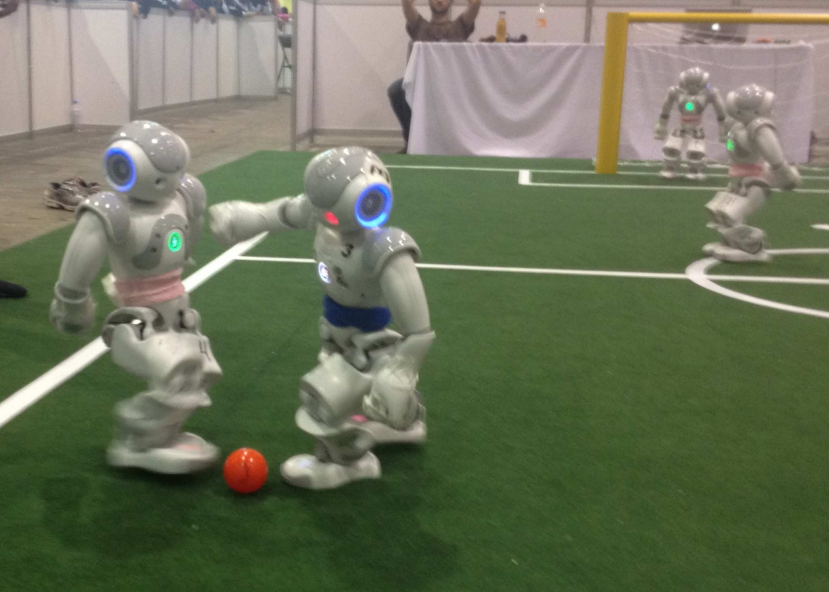
\includegraphics[width=0.7\columnwidth]{Robocup.png}
\caption{Robots play soccer. \cite{LNAI12-Barrett}}
\label{fig:robocup}
\end{figure}

However, robots can learn the action model and the 	sensor model
simultaneously without any prior knowledge. One example of such
learning is the ASAMI
algorithm \cite{CSJ06}. In the algorithm, there are two estimates of the current state
of the robot --- $W_s$, the state estimated by the sensor model, and
$W_a$, the state estimated by the action model. They are both assumed
to be polynomial functions, and the robot needs to estimate the parameters
of each estimate. In a one-dimensional scenario, the robot is required
to walk back and forth (which clearly requires some knowledge of the
actions).  In one iteration, the action model is used to update the
sensor model, and vice verse. They will finally converge in a
bootstrapping way. This idea is illustrated in
Figure~\ref{fig:relation}.

\begin{figure}
\centering
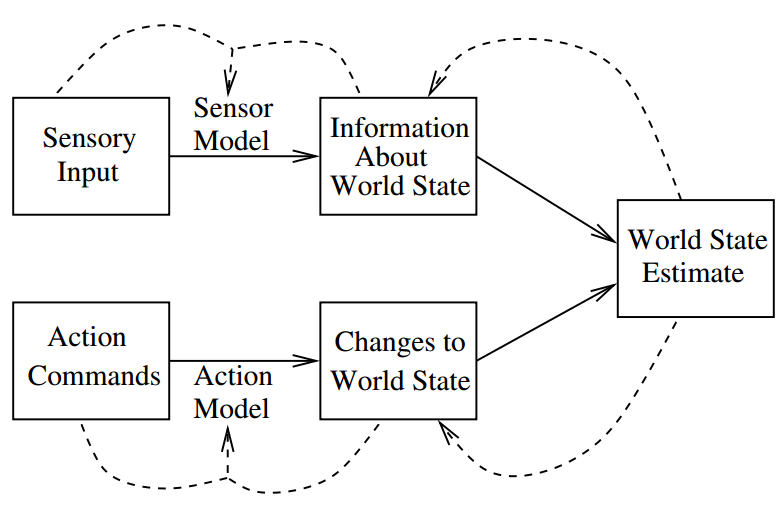
\includegraphics[width=0.7\columnwidth]{relation.png}
\caption{the robot can use redundant information to learn its action
and sensor models, revised from Figure~2 in \cite{CSJ06}.}
\label{fig:relation}
\end{figure}

\section{Analysis of ASAMI}

In ASAMI, actions are selected randomly
in the training. However, this can be biased according to the current
belief.  In this sense, the agent should be able to determine which
action would lead to the most uncertain results and thus need more
samples.  It
only knows the consistency of them, and has no knowledge about the
correctness of the models. For example, states with a larger
difference in the action model and the sensor model ($|W_a - W_s|$) should be
considered inconsistent.  For unobserved state, action pairs can be
also assumed to be inconsistent.

The first author of \cite{CSJ06}, Dan Stronger, commented that ``one
possible reason the $W_a$ is wrong after a certain action is that the
action is just very noisy \ldots This is a good reason to gather more
data for that action \ldots  But another possible reason  an action
could be causing problems is because the action model function being
fit, with the degrees of freedom that it has, just fits to a function
that's not especially accurate for that action''. This would be a
problem in degree selection in the polynomial regression
\cite{IJAIT08-stronger}. In this paper, I'll give our action model
proper degrees of freedom. So, if the action model is inconsistent,
the reason should be that either there are too few data gathered to
make consistency happen, or the data gathered are too noisy.

Action selection is even necessary in some environment. The
experiments in \cite{CSJ06} assume that \textit{we} know the effects of
the actions (going forward, going backward, etc.).
So to explore the environment, we make the robot walk forward and
backward alternatively to explore the state space. However, 
the actions' effects may be completely unknown.  If the agent still
chooses the actions uniformly random, then exploration would be
inefficient.

For example, we consider one-dimensional walk. Let the world be in the
range of $[0,n]$. The agent starts at 0, and wants to reach $n$. Let
the range of velocity be $[-2a, 2a]$ (positive velocities mean going
forward, and negative ones mean going backward), and in every step the
agent chooses an action uniformly random. Under these conditions, the expected absolute
velocity of the walk is $a$. Assume the agent would ``bump into'' the boundary of
$0$ and stays there if it tries to go backward from position $0$. The
expected \textit{moving forward} steps needed to take to reach
position $n$ from $0$ is $\frac{n}{a}$. This forms a \textit{random walk}
\cite{motwani1995randomized} problem. The expected steps needed to
take to reach distance $n$ is $O(n^2)$. This implies that if an
agent takes random actions in an unknown domain, it is likely that the
agent would restrict itself within a small sub-domain.

\section{Literature Review}

In the perspective of model-adaptive agents \cite{maes1993modeling},
\textit{action selection} is a critical problem because it
accelerates the progress towards its goal---consistency between the action
model and the transition model. This also solves the problem of
\textit{learning from experience}, as the inconsistency is an
essential piece of information that can be used for further decision-making.

There is a two-dimensional version of ASAMI discussed in
\cite{ICRA08-stronger}.  As the action space is larger in higher
dimensions, biasing on actions instead of random selection on actions
becomes more essential.

Compared with this proposed method, some similar ideas are discussed
in the developmental robotics literature. They call the inconsistency
described above as \textit{error} \cite{oudeyer2006discovering},
\textit{surprise} \cite{ranasinghe2008surprise} or \textit{curiosity}
\cite{schmidhuber2006developmental}. This serves as a motivation to
change the model. A metric can be used to describe the global
inconsistency \cite{oudeyer2006discovering}. Then, a reinforcement
learning framework can be used to plan to get to the states with the
least global inconsistency. The authors in
\cite{ranasinghe2008surprise} used logic rules as the model, and let
the robot figure out why there could be a surprise. In this paper, I
assume that the surprise is caused by insufficient or noisy data. So
the surprise, or inconsistency, of an action, is simply caused by the
data gathered at that action.

Additionally, there is an assumption in \cite{CSJ06} that there is a
mapping from action to the difference of state, i.e., $A \rightarrow
\Delta S$, where $A$ is the action space and $S$ is the state space.  This
is true in robot motion. So it's possible to learn the difference of
the states, when an action is given. This is
exactly how the task is designed in \cite{ICDL10-hester}. If this is
not true, so that $S \times A \rightarrow S$ is the best we can
estimate, this would become more challenging but still possible to be
dealt with. We might know that a certain $(s, a)$ is inconsistent and
we want to gather more data on it. But our action model might not be
well-learned, so the reward should be a compromise between the
inconsistency of that $(s, a)$ and the cost to reach it.

There are also other related works on learning the action model, but
they make use of very different approaches. They assume that one model,
usually the sensor model, is well calibrated. The data are represented
as either statistics \cite{And_learningand} or instances
\cite{LNAI2007-ahmadi}. These methods would be further analyzed and
compared with our approach in Section~\ref{sec:dis}.

\section{Proposed Algorithm}

\begin{algorithm*}
\caption{Strong ASAMI}\label{alg:asami}
\begin{algorithmic}[1]
\Function{initialize}{$rangeOfActions$}
    \State $trials\gets 0$
    \State $actions \gets$ discretized $rangeOfActions$
    \For{$action$ in $actions$}
        \State $samples[action] \gets \{\}$ \label{asa:actInit}
	\Comment{Initialize a sample set for each action}
        \State $s \gets A_0(action)$
	\State push $s$ to $samples[action]$
	\Comment{add the prediction by the initial action model}
    \EndFor
\EndFunction
\\
\Function{update}{$action, \Delta state$} \label{asa:update}
    \State add $\Delta state$ to $samples[action]$
    \State increase $trials$
\EndFunction
\\
\Function{getAction}{} \label{asa:getAct}
    \If {$trials\leq$ ACTION\_LEARNING\_TRIALS}
        \State $action \gets$ the action such that $samples[action]$ has the largest variance
    \Else
        \State $action \gets$ appropriate action for state exploration \label{asa:actSel2}
    \EndIf
\EndFunction
\end{algorithmic}
\end{algorithm*}

In this section, I propose an algorithm, named Strong ASAMI,
which makes the agent choose actions in a computationally cheap way.
It keeps the essentials of ASAMI, however, Strong ASAMI can be applied
when there is no prior domain knowledge about the action model. The
idea is that we divide the learning process into two phases. The agent
learns the actions first and learns the state space later. In the
first phase, it chooses the action with least confidence to learn. In
the second phase, it uses the actions it learned to explore the
environment.

Some essential functions are presented in Algorithm~\ref{alg:asami}.
In initialization, a sample list is initialized for each action
(Line~\ref{asa:actInit}). $A_0$ is the initial action model (a roughly
correct action model we have), and its prediction for each action is
pushed to the corresponding sample list.  This is a useful
initialization, as the variance of the sample list would represent
the error of our initial model, when the first observed sample is
added.

In each iteration, \texttt{update} (Line~\ref{asa:update}) is called to update
the knowledge of the action effects by adding new observations. When
the robot needs to decide what action to take next,
\texttt{getAction} (Line~\ref{asa:getAct}) is called.
The action selection strategy in phase 2 (Line~\ref{asa:actSel2}) is
quite vague. However, this is up to the agent to decide how to plan to traverse
the state space. Consider a one-dimensional environment, it might want
to keep trying actions with positive $\Delta state$. When it observes
no state changes after executing such action, then it tries actions
with negative $\Delta state$. With this, the robot should have the
performance of walking forward and backward in the domain.

\section{Experiments}

The setup used in my experiment is the same setup used to evaluate
ASAMI \cite{CSJ06}. The
plan for the experimental evaluation is detailed below.
Firstly, the robot can walk back and forth in a one-dimensional path.
There is a beacon placed at one end, and the robot is always facing
towards the beacon. The only observation is the height of the beacon.
The state is given by the distance to the beacon
(Figure~\ref{fig:env}).  The environment could be noisy - this is
inherently true when doing experiment on real robots.

\begin{figure}
\centering
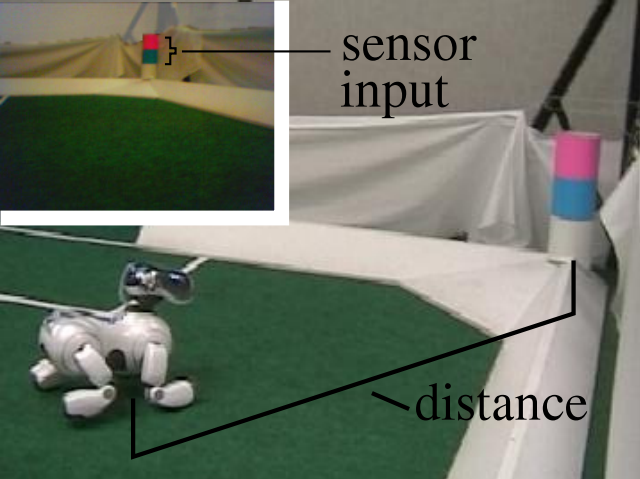
\includegraphics[width=0.6\columnwidth]{env.png}
\caption{The observation is the height of the beacon in the experiment.
The state is the distance to the beacon. Nao is used instead of Aibo
shown in this figure. \cite{CSJ06}}
\label{fig:env}
\end{figure}

First, I test ASAMI in a toy domain. I only naively implemented the action
model and the sensor model. Then, I made ASAMI and Strong ASAMI work on
Aldebaran Nao robot. Action model and sensor model are both assumed to be cubic
functions, and we have four parameters to estimate for each model. The
initial action model $A_0$ is defined to be a constant function,
$A_0(x) = c$, where c is a small random number. This is used to train
the state estimated by the action model $w_a$ in the first 100
iterations.

The goal is to have $W_s$ and $W_a$ both converge and consistent with
the true position, or state. It is possible that they are not
numerically equal to the state, but they should have the same shape,
that is, they could be an offset or scale of the true function.

\subsection{Test in Simulator}

\begin{figure}
\centering
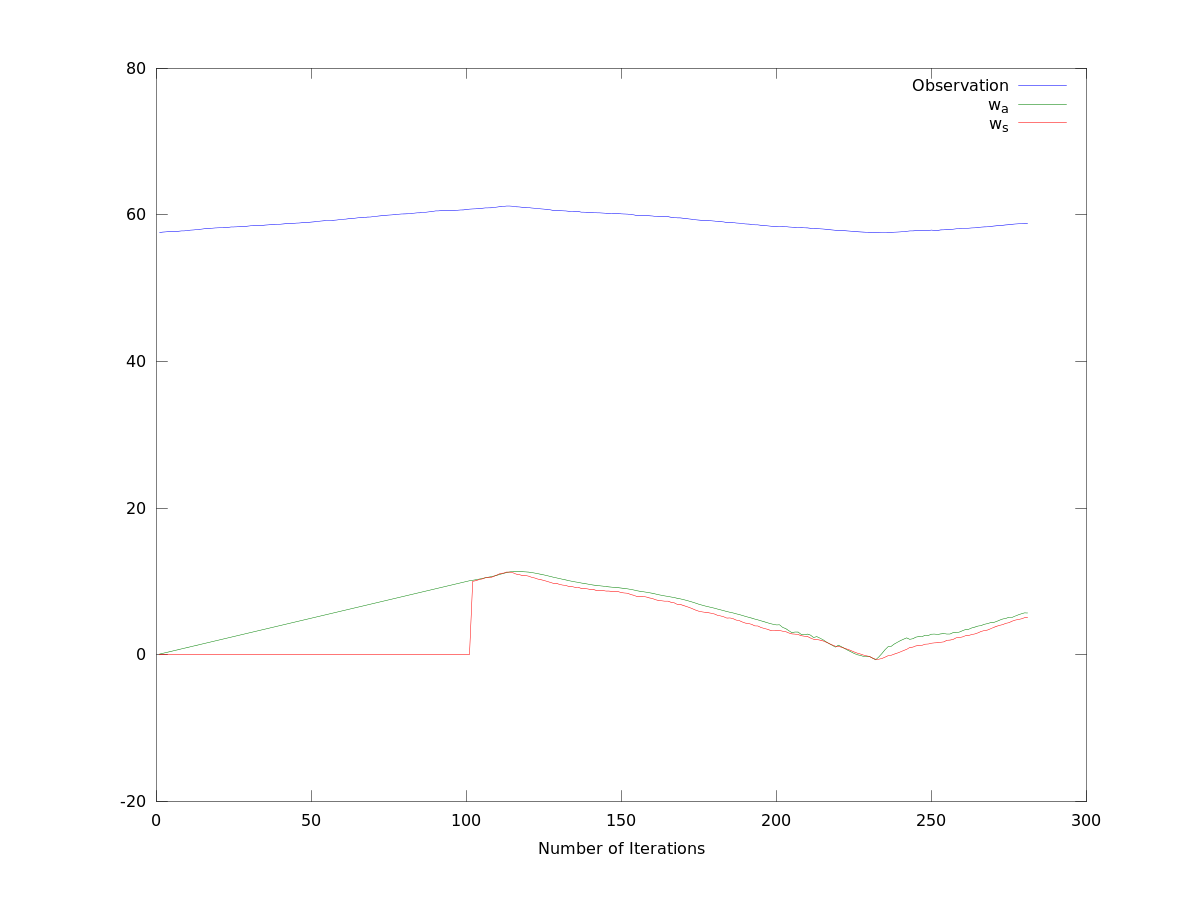
\includegraphics[width=0.7\columnwidth]{simResult.png}
\caption{The learning performance in the simulator.}
\label{fig:sim}
\end{figure}

The actions in the simulator are simply walking backward or froward.
The robot can choose from velocity of [-1, 1]. The change of state is
affected by the velocity.
The sensor model computes the height of the beacon according to the
current state. The result is in Figure~\ref{fig:sim}. There is no
noise in the simulator so the results show that the learning on both
models converge quickly. Estimates from both models have the same
shape as the true states.

\subsection{Test on Nao: First Attempt}
\label{nao:1st}

The challenges of making ASAMI walk on Nao are that beacon height is
too noisy, the height returned by the beacon detector could be noisy
because the observed image can blur, and the real walking velocity can
be different from what is set. The result is in Figure~\ref{fig:demo}.

The observation is retrieved and ASAMI is updated in each iteration.
The beacon height shows that the robot walks forward and backward two
times, and then kidnapped\footnote{Kidnapping means that while the robot
is walking, you quickly put it to a different position. The robot
would find its environment changes unpredictably, then it realizes its
location changed.} from a further point to a closer point to
the beacon in around 3,500 iteration.

\begin{figure}[h]
\centering
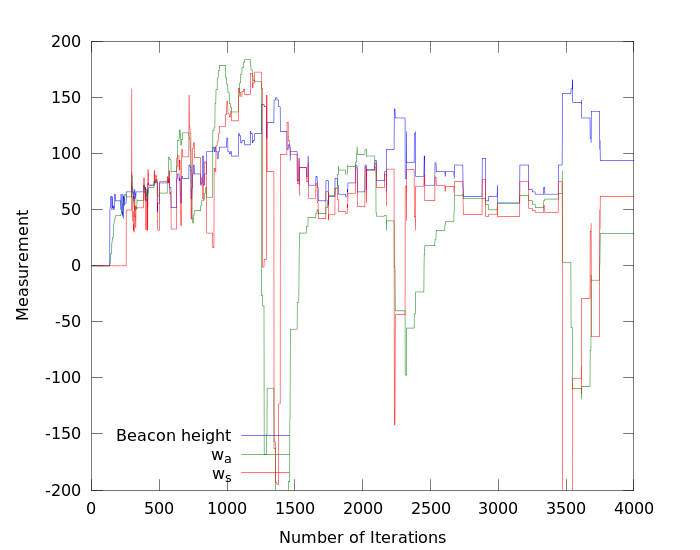
\includegraphics[width=0.7\columnwidth]{demoResult.png}
\caption{Testing of ASAMI on Nao during the class demo. The
observation comes continuously, on average of 30 frames (iterations)
per second. It is kidnapped at around 3,500th iteration.}
\label{fig:demo}
\end{figure}

\subsection{Test on Nao: Second Attempt}

\begin{figure}[h]
\centering
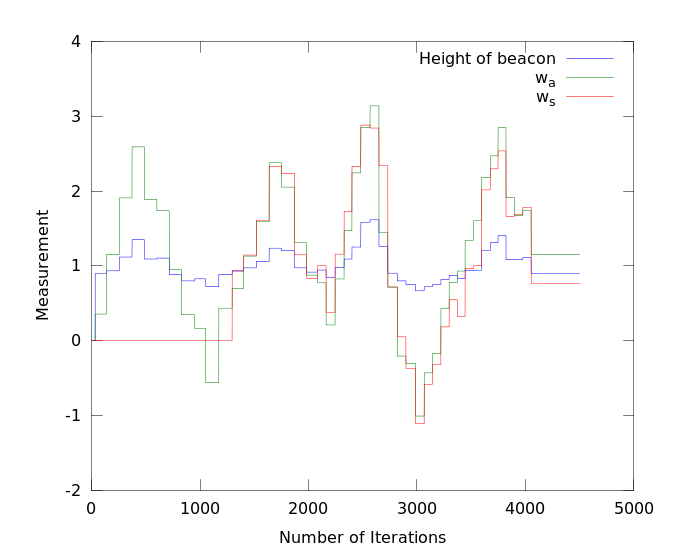
\includegraphics[width=0.7\columnwidth]{out_obs.png}
\caption{Testing of ASAMI on Nao. The observation comes only when it's
in standing phase. So there is less update in the observation, and
less noise compared to Figure~\ref{fig:demo}. One iteration of ASAMI
corresponds to one update in the figure, which corresponding to many
frames on Nao (I re-scaled the height of beacon, so that they can be
plotted in a same magnitude).}
\label{fig:obs}
\end{figure}

I realized that making Nao observe while walking is not necessary, so
I made the Nao observe while stationary.
During the test, Nao will take an action, walk, and then stand still
to observe the beacon.
 It keeps repeating
this sequence. The result is in Figure~\ref{fig:obs}.  The 
beacon height in the figure is the average of the observed beacon heights in
the standing phase. Note that the x label in Figure~\ref{fig:obs} is
different from that in Figure~\ref{fig:demo}. In Figure~\ref{fig:demo},
one iteration of ASAMI is exactly one frame on Nao. Here, one
iteration of ASAMI takes many frames on Nao (one walking and one
standing phase).

Clearly, as there are less noise in the observation, the data are more
accurate. ASAMI has a better performance.

\subsection{Test on Nao: using Strong ASAMI}

\begin{figure}[h]
\centering
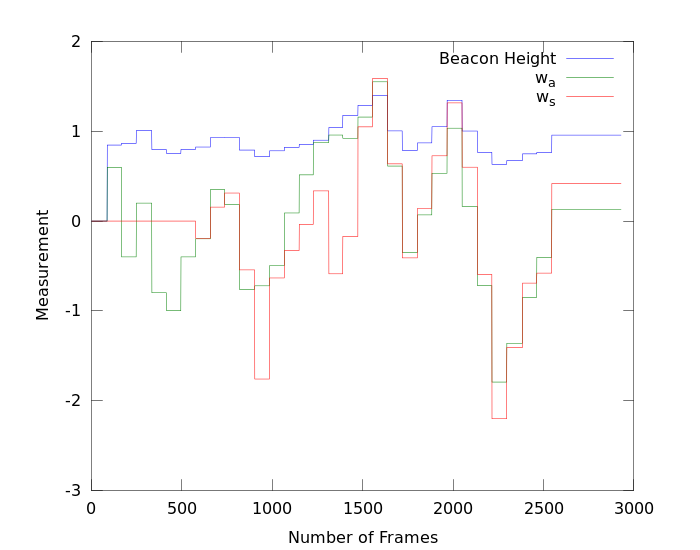
\includegraphics[width=0.7\columnwidth]{out_strong.png}
\caption{Testing of Strong ASAMI on Nao. The observation comes only
when it's in standing phase - same as Figure~\ref{fig:obs}. The robot
tries to learn the action model first in the first 1,500 iterations,
then continues to explore the state space (I re-scaled the height of
beacon, so that they can be plotted in a same magnitude).}
\label{fig:obs_strong}
\end{figure}

Strong ASAMI is applied in this experiment. The assumption is
different from the previous ones - Nao doesn't have the knowledge of
the actions. The results are in Figure~\ref{fig:obs_strong}. The
beacon height shows that the robot tries different actions
first (within 1,500 iterations, or frames) and then moves forward and
backward to explore the state space.

Another intended goal is to show that convergence in
Figure~\ref{fig:obs_strong} should be faster than that in previous
experiments. Actually, the difference is not significant, at least for
one-dimensional environment.

\section{Discussion and Conclusion}
\label{sec:dis}

The idea of action trials is very similar to the idea of N-bandit
problem \cite{vermorel2005multi}. In N-bandit problem, we choose one
action at each step, with the objective to maximize the overall
rewards. However, the goal of our problem is to minimize
the variance of all the actions. To solve this problem, I used a 
approach of 
choosing an action with the largest variance at each step. The
experiments have shown that this approach worked, even though there is
room for improvement. For example, as the actions are
not mutually independent - they are picked up from a continuous space,
getting one sample of an action can help us know its neighborhood.

We assume the action space as a continuous space in the experiments.
However, it is possible that learning each discrete action independently would
have a better performance (same metric as
\cite{LNAI2007-ahmadi}). The action model and the sensor model are
both assumed to be polynomial function in the experiments, but it has
several constraints. First, degree selection should be
determined, possibly using methods in \cite{IJAIT08-stronger}. But the
model may not be a small-dimensional polynomial, so there might be
too many parameters to estimate. Second, the inherent limitation of
function approximation method is that local updates could have global
effects. This is especially harmful in a noisy environment.

% The action model and sensor model are comparatively easy to learn for
% a one-dimensional environment. So expecting improvement on the
% result of ASAMI algorithm may not be realistic. However,
In this report, I show that Strong ASAMI shows its power in the
environment where action learning is necessary. This is just for
one-dimensional environment. So future work can be extending to
testing in multi-dimensional environments.

\section{Acknowledgment}

This paper is revised from the report of the final project in
Autonomous Robots class,
instructed by Prof. Peter Stone, Department of Computer Science. He
gave me valuable advices on this research. The first author of
\cite{CSJ06}, Dan Stronger, also gave me comments when I proposed this
project.

%=====================================================================
\bibliographystyle{plain}

\bibliography{report}

\end{document}
